%  LaTeX support: latex@mdpi.com 
%  For support, please attach all files needed for compiling as well as the log file, and specify your operating system, LaTeX version, and LaTeX editor.

\newcommand{\qsdpapertitle}{Inertia and Motion Under the Substrate Response: A Structural Interpretation of Reconfiguration and Delay}
\newcommand{\qsdauthorname}{Michael Bush}
\newcommand{\qsdauthorinitials}{M.B.}
\newcommand{\qsdauthoremail}{mbush@haddentechnologies.com}
\newcommand{\qsdorcid}{0009-0003-9747-9109}
\newcommand{\qsdcorp}{Hadden Technologies Corporation}
\newcommand{\qsdgptname}{ChatGPT}
\newcommand{\qsdgptver}{GPT-4o}
\newcommand{\qsdgptyear}{2025}
\newcommand{\qsdkeywords}{Inertia,Scalar coherence,Substrate dynamics  
Quantum Substrate Dynamics,QSD,Phase re-locking,Structural,motion,Momentum,Rotational loss,Lorentz invariance,Inertial symmetry,Scalar recovery,Mass-phase structure,Conserved substrate}
\newcommand{\qsdmethodstatement}
{This work was developed through first-principles modeling using a conserved coherence substrate framework. All derivations were performed structurally, with motion, inertia, and rotational behavior treated as manifestations of scalar phase reconfiguration. Mathematical relationships were constructed to maintain causal consistency and empirical compatibility, while avoiding reliance on classical axioms such as intrinsic mass or force. The method emphasizes substrate conservation, phase continuity, and Lorentz-invariant scalar timing to reveal the structural origins of inertial and dynamic behavior.}
\newcommand{\qsdabstract}
{This paper presents a structural reinterpretation of motion, inertia, and momentum within the framework of Quantum Substrate Dynamics (QSD), a conserved, coherence-based model of mass and interaction. We begin by examining the fundamental nature of velocity and inertial resistance, demonstrating that motion is not spatial traversal but a scalar-guided process of substrate phase re-locking. In this view, inertia emerges as the energetic cost of deforming a mass-phase coherence boundary, and momentum is understood as the substrate’s accumulated commitment to a coherence reconfiguration trajectory.\\
We show that uniform linear motion corresponds to tension-neutral substrate flow, while acceleration, deceleration, and rotation all require scalar recovery work — producing observable thermal and kinetic signatures. Rotational motion is shown to be inherently lossy due to persistent phase curvature, and gyroscopic resistance is derived directly from the substrate’s conservation of angular coherence memory. Weight is reframed as local scalar tension pushback, experienced when coherence structures are held out of equilibrium in a tension gradient. These insights resolve Einstein’s inertial frame equivalence from first principles, while preserving Lorentz invariance and classical conservation laws.\\
No legacy physics principles are violated; instead, this framework reveals the structural origins of classical laws. Motion, inertia, and momentum emerge not from force or mass, but from substrate geometry, tension conservation, and scalar timing. The result is a coherent, falsifiable, and physically intuitive model of motion rooted in a deeper ontology — one which invites future applications in coherent transport, scalar-assisted motion, and structural sensing.}

%=================================================================
\documentclass[entropy,article,submit,pdftex,moreauthors]{Definitions/mdpi} 
%\documentclass[preprints,article,submit,pdftex,moreauthors]{Definitions/mdpi} 
% For posting an early version of this manuscript as a preprint, you may use "preprints" as the journal. Changing "submit" to "accept" before posting will remove line numbers.

% Below journals will use APA reference format:
% admsci, aieduc, behavsci, businesses, econometrics, economies, education, ejihpe, famsci, games, humans, ijcs, ijfs, journalmedia, jrfm, languages, psycholint, publications, tourismhosp, youth

% Below journals will use Chicago reference format:
% arts, genealogy, histories, humanities, jintelligence, laws, literature, religions, risks, socsci

%--------------------
% Class Options:
%--------------------
%----------
% journal
%----------
% Choose between the following MDPI journals:
% accountaudit, acoustics, actuators, addictions, adhesives, admsci, adolescents, aerobiology, aerospace, agriculture, agriengineering, agrochemicals, agronomy, ai, air, algorithms, allergies, alloys, amh, analytica, analytics, anatomia, anesthres, animals, antibiotics, antibodies, antioxidants, applbiosci, appliedchem, appliedmath, appliedphys, applmech, applmicrobiol, applnano, applsci, aquacj, architecture, arm, arthropoda, arts, asc, asi, astronomy, atmosphere, atoms, audiolres, automation, axioms, bacteria, batteries, bdcc, behavsci, beverages, biochem, bioengineering, biologics, biology, biomass, biomechanics, biomed, biomedicines, biomedinformatics, biomimetics, biomolecules, biophysica, biosensors, biosphere, biotech, birds, blockchains, bloods, blsf, brainsci, breath, buildings, businesses, cancers, carbon, cardiogenetics, catalysts, cells, ceramics, challenges, chemengineering, chemistry, chemosensors, chemproc, children, chips, cimb, civileng, cleantechnol, climate, clinbioenerg, clinpract, clockssleep, cmd, cmtr, coasts, coatings, colloids, colorants, commodities, complications, compounds, computation, computers, condensedmatter, conservation, constrmater, cosmetics, covid, crops, cryo, cryptography, crystals, csmf, ctn, curroncol, cyber, dairy, data, ddc, dentistry, dermato, dermatopathology, designs, devices, diabetology, diagnostics, dietetics, digital, disabilities, diseases, diversity, dna, drones, dynamics, earth, ebj, ecm, ecologies, econometrics, economies, education, eesp, ejihpe, electricity, electrochem, electronicmat, electronics, encyclopedia, endocrines, energies, eng, engproc, ent, entomology, entropy, environments, epidemiologia, epigenomes, esa, est, famsci, fermentation, fibers, fintech, fire, fishes, fluids, foods, forecasting, forensicsci, forests, fossstud, foundations, fractalfract, fuels, future, futureinternet, futureparasites, futurepharmacol, futurephys, futuretransp, galaxies, games, gases, gastroent, gastrointestdisord, gastronomy, gels, genealogy, genes, geographies, geohazards, geomatics, geometry, geosciences, geotechnics, geriatrics, glacies, grasses, greenhealth, gucdd, hardware, hazardousmatters, healthcare, hearts, hemato, hematolrep, heritage, higheredu, highthroughput, histories, horticulturae, hospitals, humanities, humans, hydrobiology, hydrogen, hydrology, hygiene, idr, iic, ijerph, ijfs, ijgi, ijmd, ijms, ijns, ijpb, ijt, ijtm, ijtpp, ime, immuno, informatics, information, infrastructures, inorganics, insects, instruments, inventions, iot, j, jal, jcdd, jcm, jcp, jcs, jcto, jdad, jdb, jeta, jfb, jfmk, jimaging, jintelligence, jlpea, jmahp, jmmp, jmms, jmp, jmse, jne, jnt, jof, joitmc, joma, jop, jor, journalmedia, jox, jpbi, jpm, jrfm, jsan, jtaer, jvd, jzbg, kidney, kidneydial, kinasesphosphatases, knowledge, labmed, laboratories, land, languages, laws, life, lights, limnolrev, lipidology, liquids, literature, livers, logics, logistics, lubricants, lymphatics, machines, macromol, magnetism, magnetochemistry, make, marinedrugs, materials, materproc, mathematics, mca, measurements, medicina, medicines, medsci, membranes, merits, metabolites, metals, meteorology, methane, metrics, metrology, micro, microarrays, microbiolres, microelectronics, micromachines, microorganisms, microplastics, microwave, minerals, mining, mmphys, modelling, molbank, molecules, mps, msf, mti, multimedia, muscles, nanoenergyadv, nanomanufacturing, nanomaterials, ncrna, ndt, network, neuroglia, neurolint, neurosci, nitrogen, notspecified, nursrep, nutraceuticals, nutrients, obesities, oceans, ohbm, onco, oncopathology, optics, oral, organics, organoids, osteology, oxygen, parasites, parasitologia, particles, pathogens, pathophysiology, pediatrrep, pets, pharmaceuticals, pharmaceutics, pharmacoepidemiology, pharmacy, philosophies, photochem, photonics, phycology, physchem, physics, physiologia, plants, plasma, platforms, pollutants, polymers, polysaccharides, populations, poultry, powders, preprints, proceedings, processes, prosthesis, proteomes, psf, psych, psychiatryint, psychoactives, psycholint, publications, purification, quantumrep, quaternary, qubs, radiation, reactions, realestate, receptors, recycling, regeneration, religions, remotesensing, reports, reprodmed, resources, rheumato, risks, robotics, rsee, ruminants, safety, sci, scipharm, sclerosis, seeds, sensors, separations, sexes, signals, sinusitis, siuj, skins, smartcities, sna, societies, socsci, software, soilsystems, solar, solids, spectroscj, sports, standards, stats, std, stresses, surfaces, surgeries, suschem, sustainability, symmetry, synbio, systems, tae, targets, taxonomy, technologies, telecom, test, textiles, thalassrep, therapeutics, thermo, timespace, tomography, tourismhosp, toxics, toxins, transplantology, transportation, traumacare, traumas, tropicalmed, universe, urbansci, uro, vaccines, vehicles, venereology, vetsci, vibration, virtualworlds, viruses, vision, waste, water, wem, wevj, wild, wind, women, world, youth, zoonoticdis

%---------
% article
%---------
% The default type of manuscript is "article", but can be replaced by: 
% abstract, addendum, article, benchmark, book, bookreview, briefcommunication, briefreport, casereport, changes, clinicopathologicalchallenge, comment, commentary, communication, conceptpaper, conferenceproceedings, correction, conferencereport, creative, datadescriptor, discussion, entry, expressionofconcern, extendedabstract, editorial, essay, erratum, fieldguide, hypothesis, interestingimages, letter, meetingreport, monograph, newbookreceived, obituary, opinion, proceedingpaper, projectreport, reply, retraction, review, perspective, protocol, shortnote, studyprotocol, supfile, systematicreview, technicalnote, viewpoint, guidelines, registeredreport, tutorial,  giantsinurology, urologyaroundtheworld
% supfile = supplementary materials

%----------
% submit
%----------
% The class option "submit" will be changed to "accept" by the Editorial Office when the paper is accepted. This will only make changes to the frontpage (e.g., the logo of the journal will get visible), the headings, and the copyright information. Also, line numbering will be removed. Journal info and pagination for accepted papers will also be assigned by the Editorial Office.

%------------------
% moreauthors
%------------------
% If there is only one author the class option oneauthor should be used. Otherwise use the class option moreauthors.

%---------
% pdftex
%---------
% The option pdftex is for use with pdfLaTeX. Remove "pdftex" for (1) compiling with LaTeX & dvi2pdf (if eps figures are used) or for (2) compiling with XeLaTeX.

%=================================================================
% MDPI internal commands - do not modify
\firstpage{1} 
\makeatletter 
\setcounter{page}{\@firstpage} 
\makeatother
\pubvolume{1}
\issuenum{1}
\articlenumber{0}
\pubyear{2025}
\copyrightyear{2025}
%\externaleditor{Firstname Lastname} % More than 1 editor, please add `` and '' before the last editor name
\datereceived{ } 
\daterevised{ } % Comment out if no revised date
\dateaccepted{ } 
\datepublished{ } 
%\datecorrected{} % For corrected papers: "Corrected: XXX" date in the original paper.
%\dateretracted{} % For retracted papers: "Retracted: XXX" date in the original paper.
\hreflink{https://doi.org/} % If needed use \linebreak
%\doinum{}
%\pdfoutput=1 % Uncommented for upload to arXiv.org
%\CorrStatement{yes}  % For updates
%\longauthorlist{yes} % For many authors that exceed the left citation part

%=================================================================
% Add packages and commands here. The following packages are loaded in our class file: fontenc, inputenc, calc, indentfirst, fancyhdr, graphicx, epstopdf, lastpage, ifthen, float, amsmath, amssymb, lineno, setspace, enumitem, mathpazo, booktabs, titlesec, etoolbox, tabto, xcolor, colortbl, soul, multirow, microtype, tikz, totcount, changepage, attrib, upgreek, array, tabularx, pbox, ragged2e, tocloft, marginnote, marginfix, enotez, amsthm, natbib, hyperref, cleveref, scrextend, url, geometry, newfloat, caption, draftwatermark, seqsplit
% cleveref: load \crefname definitions after \begin{document}

\usepackage{tikz}
\usetikzlibrary{angles, quotes}
\usepackage{pgfplots}
\pgfplotsset{compat=1.17}

%=================================================================
% Please use the following mathematics environments: Theorem, Lemma, Corollary, Proposition, Characterization, Property, Problem, Example, ExamplesandDefinitions, Hypothesis, Remark, Definition, Notation, Assumption
%% For proofs, please use the proof environment (the amsthm package is loaded by the MDPI class).

%=================================================================
% Full title of the paper (Capitalized)
\Title{\qsdpapertitle}


% MDPI internal command: Title for citation in the left column
\TitleCitation{Title}

% Author Orchid ID: enter ID or remove command
\newcommand{\orcidauthorA}{\qsdorcid} % Add \orcidA{} behind the author's name
%\newcommand{\orcidauthorB}{0000-0000-0000-000X} % Add \orcidB{} behind the author's name

% Authors, for the paper (add full first names)
\Author{\qsdauthorname $^{1}$\orcidA{}}

%\longauthorlist{yes}

% MDPI internal command: Authors, for metadata in PDF
\AuthorNames{\qsdauthorname}

% MDPI internal command: Authors, for citation in the left column, only choose below one of them according to the journal style
% If this is a Chicago style journal 
% (arts, genealogy, histories, humanities, jintelligence, laws, literature, religions, risks, socsci): 
% Lastname, Firstname, Firstname Lastname, and Firstname Lastname.

% If this is a APA style journal 
% (admsci, behavsci, businesses, econometrics, economies, education, ejihpe, games, humans, ijfs, journalmedia, jrfm, languages, psycholint, publications, tourismhosp, youth): 
% Lastname, F., Lastname, F., \& Lastname, F.

% If this is a ACS style journal (Except for the above Chicago and APA journals, all others are in the ACS format): 
% Lastname, F.; Lastname, F.; Lastname, F.
\isAPAStyle{%
       \AuthorCitation{Lastname, F., Lastname, F., \& Lastname, F.}
         }{%
        \isChicagoStyle{%
        \AuthorCitation{Lastname, Firstname, Firstname Lastname, and Firstname Lastname.}
        }{
        \AuthorCitation{Lastname, F.; Lastname, F.; Lastname, F.}
        }
}

% Affiliations / Addresses (Add [1] after \address if there is only one affiliation.)
\address{%
$^{1}$ \quad \qsdcorp; \qsdauthoremail\\
%$^{2}$ \quad Affiliation 2; e-mail@e-mail.com
}

% Contact information of the corresponding author
\corres{Correspondence: \qsdauthoremail (\qsdauthorinitials)}

% Current address and/or shared authorship
%\firstnote{Shiloh, IL: Independent Researcher.}  % Current address should not be the same as any items in the Affiliation section.
%\secondnote{These authors contributed equally to this work.}
% The commands \thirdnote{} till \eighthnote{} are available for further notes

%\simplesumm{} % Simple summary

%\conference{} % An extended version of a conference paper


% Abstract (Do not insert blank lines, i.e. \\) 
\abstract{\qsdabstract}

% Keywords
\keyword{\qsdkeywords} 

% The fields PACS, MSC, and JEL may be left empty or commented out if not applicable
%\PACS{J0101}
%\MSC{}
%\JEL{}

%%%%%%%%%%%%%%%%%%%%%%%%%%%%%%%%%%%%%%%%%%
% Only for the journal Diversity
%\LSID{\url{http://}}

%%%%%%%%%%%%%%%%%%%%%%%%%%%%%%%%%%%%%%%%%%
% Only for the journal Applied Sciences
%\featuredapplication{Authors are encouraged to provide a concise description of the specific application or a potential application of the work. This section is not mandatory.}
%%%%%%%%%%%%%%%%%%%%%%%%%%%%%%%%%%%%%%%%%%

%%%%%%%%%%%%%%%%%%%%%%%%%%%%%%%%%%%%%%%%%%
% Only for the journal Data
%\dataset{DOI number or link to the deposited data set if the data set is published separately. If the data set shall be published as a supplement to this paper, this field will be filled by the journal editors. In this case, please submit the data set as a supplement.}
%\datasetlicense{License under which the data set is made available (CC0, CC-BY, CC-BY-SA, CC-BY-NC, etc.)}

%%%%%%%%%%%%%%%%%%%%%%%%%%%%%%%%%%%%%%%%%%
% Only for the journal BioTech, Fishes, Neuroimaging and Toxins
%\keycontribution{The breakthroughs or highlights of the manuscript. Authors can write one or two sentences to describe the most important part of the paper.}

%%%%%%%%%%%%%%%%%%%%%%%%%%%%%%%%%%%%%%%%%%
% Only for the journal Encyclopedia
%\encyclopediadef{For entry manuscripts only: please provide a brief overview of the entry title instead of an abstract.}

%%%%%%%%%%%%%%%%%%%%%%%%%%%%%%%%%%%%%%%%%%
% Only for the journal Advances in Respiratory Medicine, Future, Sensors and Smart Cities
%\addhighlights{yes}
%\renewcommand{\addhighlights}{%
%
%\noindent This is an obligatory section in ``Advances in Respiratory Medicine'', ``Future'', ``Sensors'' and ``Smart Cities”, whose goal is to increase the discoverability and readability of the article via search engines and other scholars. Highlights should not be a copy of the abstract, but a simple text allowing the reader to quickly and simplified find out what the article is about and what can be cited from it. Each of these parts should be devoted up to 2~bullet points.\vspace{3pt}\\
%\textbf{What are the main findings?}
% \begin{itemize}[labelsep=2.5mm,topsep=-3pt]
% \item First bullet.
% \item Second bullet.
% \end{itemize}\vspace{3pt}
%\textbf{What is the implication of the main finding?}
% \begin{itemize}[labelsep=2.5mm,topsep=-3pt]
% \item First bullet.
% \item Second bullet.
% \end{itemize}
%}

%%%%%%%%%%%%%%%%%%%%%%%%%%%%%%%%%%%%%%%%%%
\begin{document}
%%%%%%%%%%%%%%%%%%%%%%%%%%%%%%%%%%%%%%%%%%
% The order of the section titles is different for some journals. Please refer to the "Instructions for Authors” on the journal homepage.

%%%%%%%%%%%%%%%%%%%%%%%%%%%%%%%%%%%%%%%%%%
\section{Introduction}

Motion is one of the most foundational concepts in physics, yet its underlying nature is rarely questioned. We describe velocity, acceleration, and momentum with confidence, but do so from models that treat motion as traversal, inertia as intrinsic, and momentum as a carried quantity. These assumptions are useful---and in practice, highly predictive---but they are not explanatory. We accept that mass resists acceleration, that moving bodies remain in motion, and that rotating systems resist tilt, without asking what physical substrate enforces these behaviors.

Einstein recognized this unresolved substrate in his own way. The indistinguishable state between rest and uniform motion, and the universal character of inertial resistance, were elevated to principles---yet never mechanistically derived. Even today, inertia remains unexplained: not in the mathematical sense, but in the physical. What is resisting? Where is that resistance stored? Why is motion preserved without effort---until it changes?

This paper proposes that answers to these questions can be found not by discarding physics, but by descending beneath it. Using the framework of Quantum Substrate Dynamics (QSD)~\cite{bush2025,bush-planck-2025,bush-coherence,bush-planck-ep}, but as a process of scalar phase re-locking within a conserved coherence field. In this model, mass is not substance, but structure---a phase-stable knot in the substrate. Motion is the act of reconfiguring that structure under tension. Inertia becomes the substrate's resistance to that reconfiguration, and momentum is the measure of coherence already committed to that re-locking path.

Throughout this paper, we develop a first-principles reinterpretation of motion, inertia, and momentum using only structural conservation, scalar causality, and coherence continuity. We do not break classical laws---we show what generates them. Newton’s laws, Einstein’s relativity, and modern dynamics are recovered as surface-level summaries of deeper structural behavior. What emerges is a more intuitive, testable, and physically grounded model of motion: one that preserves everything physics has already taught us, but replaces axioms with structure and interpretation with cause.

While the framework developed here is grounded in first-principles substrate modeling, it resonates with several modern empirical domains. For example, inertial frame equivalence and gravitational time dilation effects—such as those observed in the Global Positioning System (GPS)—point to an underlying coherence-related behavior that traditional models treat geometrically~\cite{ashby-gps}. In QSD, these phenomena emerge naturally as scalar pacing and gradient alignment effects. Similarly, rotational decay and frame-dragging effects observed in gyroscopic systems~\cite{gp-b} suggest a deeper structural tension dynamic within spacetime, consistent with the substrate re-locking behavior described herein. Finally, measurable thermal dissipation in spinning bodies~\cite{rotational-heating} provides indirect evidence of scalar offload mechanisms operating below the threshold of classical friction models. These connections will be explored further in subsequent work, but they highlight the compatibility of QSD with observed phenomena traditionally explained through relativity and field theory.



%%%%%%%%%%%%%%%%%%%%%%%%%%%%%%%%%%%%%%%%%%
\section{Materials and Methods}
%%%%%%%%%%%%%%%%%%%%%%%%%%%%%%%%%%%%%%%%%%
\qsdmethodstatement
In support of the editorial process, generative AI tools—specifically OpenAI's \qsdgptname (version \qsdgptver, \qsdgptyear)—were used to assist in:
\begin{itemize}
    \item Generating illustrative figures based on the author’s conceptual framework, with iterative refinement to ensure fidelity to the substrate-based dynamics of the model,
    \item Researching, validating, and cross-referencing related scientific concepts to improve accuracy, contextual alignment, and clarity,
    \item Summarizing and formatting externally sourced material already selected by the author.
\end{itemize}

No original theoretical contributions were generated by the AI system; all scientific claims, hypotheses, derivations, and interpretations were authored and reviewed by the human researcher. The use of ChatGPT is disclosed in alignment with journal policy for transparency in the writing process.

%%%%%%%%%%%%%%%%%%%%%%%%%%%%%%%%%%%%%%%%%%
%\section{Results}

%%%%%%%%%%%%%%%%%%%%%%%%%%%%%%%%%%%%%%%%%%
\section{Discussion}
%%%%%%%%%%%%%%%%%%%%%%%%%%%%%%%%%%%%%%%%%%
\subsection{Substrate Ontology of Motion}

In the framework of Quantum Substrate Dynamics (QSD) \cite{bush2025}, motion is not interpreted as continuous traversal through an external geometric manifold, but as the re-locking of a phase-stable coherence structure within a conserved substrate \cite{bush-coherence}. The substrate is treated as a causally structured, scalar-supporting medium whose internal coherence defines mass, inertia, and displacement. In this view, the motion of a mass-phase structure occurs only when the substrate permits a successful reconfiguration of that structure’s coherence into an adjacent phase-compatible region.

From this perspective, velocity is not a primitive variable, but an emergent measure of scalar re-locking rate. A structure at rest is one whose coherence boundary remains phase-stable in its current location; a structure in uniform motion is one whose re-locking occurs at a constant rate, aligned with a tension-neutral substrate gradient. Acceleration, by contrast, reflects a directional increase in re-lock demand, resulting in scalar deformation of the boundary shell.

Space and time are no longer treated as background coordinates, but as emergent properties of the substrate's capacity to support structured coherence. Spatial displacement corresponds to the successful transfer of a coherence structure across sequential substrate regions; temporal progression arises from the scalar recovery interval required between offload and re-lock events. In this formulation, time is inherently directional, rooted in the causal pacing of coherence recovery rather than in geometric reversibility.

The substrate itself does not flow or move, and it deforms only under conserved coherence strain. It acts as a stationary, conserved scaffold for phase anchoring. Motion is not motion of matter through space, but the motion of structure through substrate permission. All classical kinematics are reinterpreted as large-scale summaries of this scalar-guided coherence realignment.

This leads naturally to the definition of a coherence transport velocity, which represents the effective speed at which a phase-locked structure can re-lock into adjacent substrate regions:

\begin{equation}
    v_{\text{coh}} = \frac{L_{\text{coh}}}{t_{\text{tick}}},
\end{equation}

where \( L_{\text{coh}} \) is the characteristic size of the coherence envelope and \( t_{\text{tick}} \) is the scalar recovery time between permissible re-locking events. This expression reflects the maximum rate of substrate-supported motion for a given structure, bounded not by traversal limits, but by local coherence and causality constraints. It replaces geometric motion with structural pacing, preserving Lorentz consistency through scalar continuity, see Figure \ref{fig:coherence-transport-velocity}.

\begin{figure}[H]
    \centering
    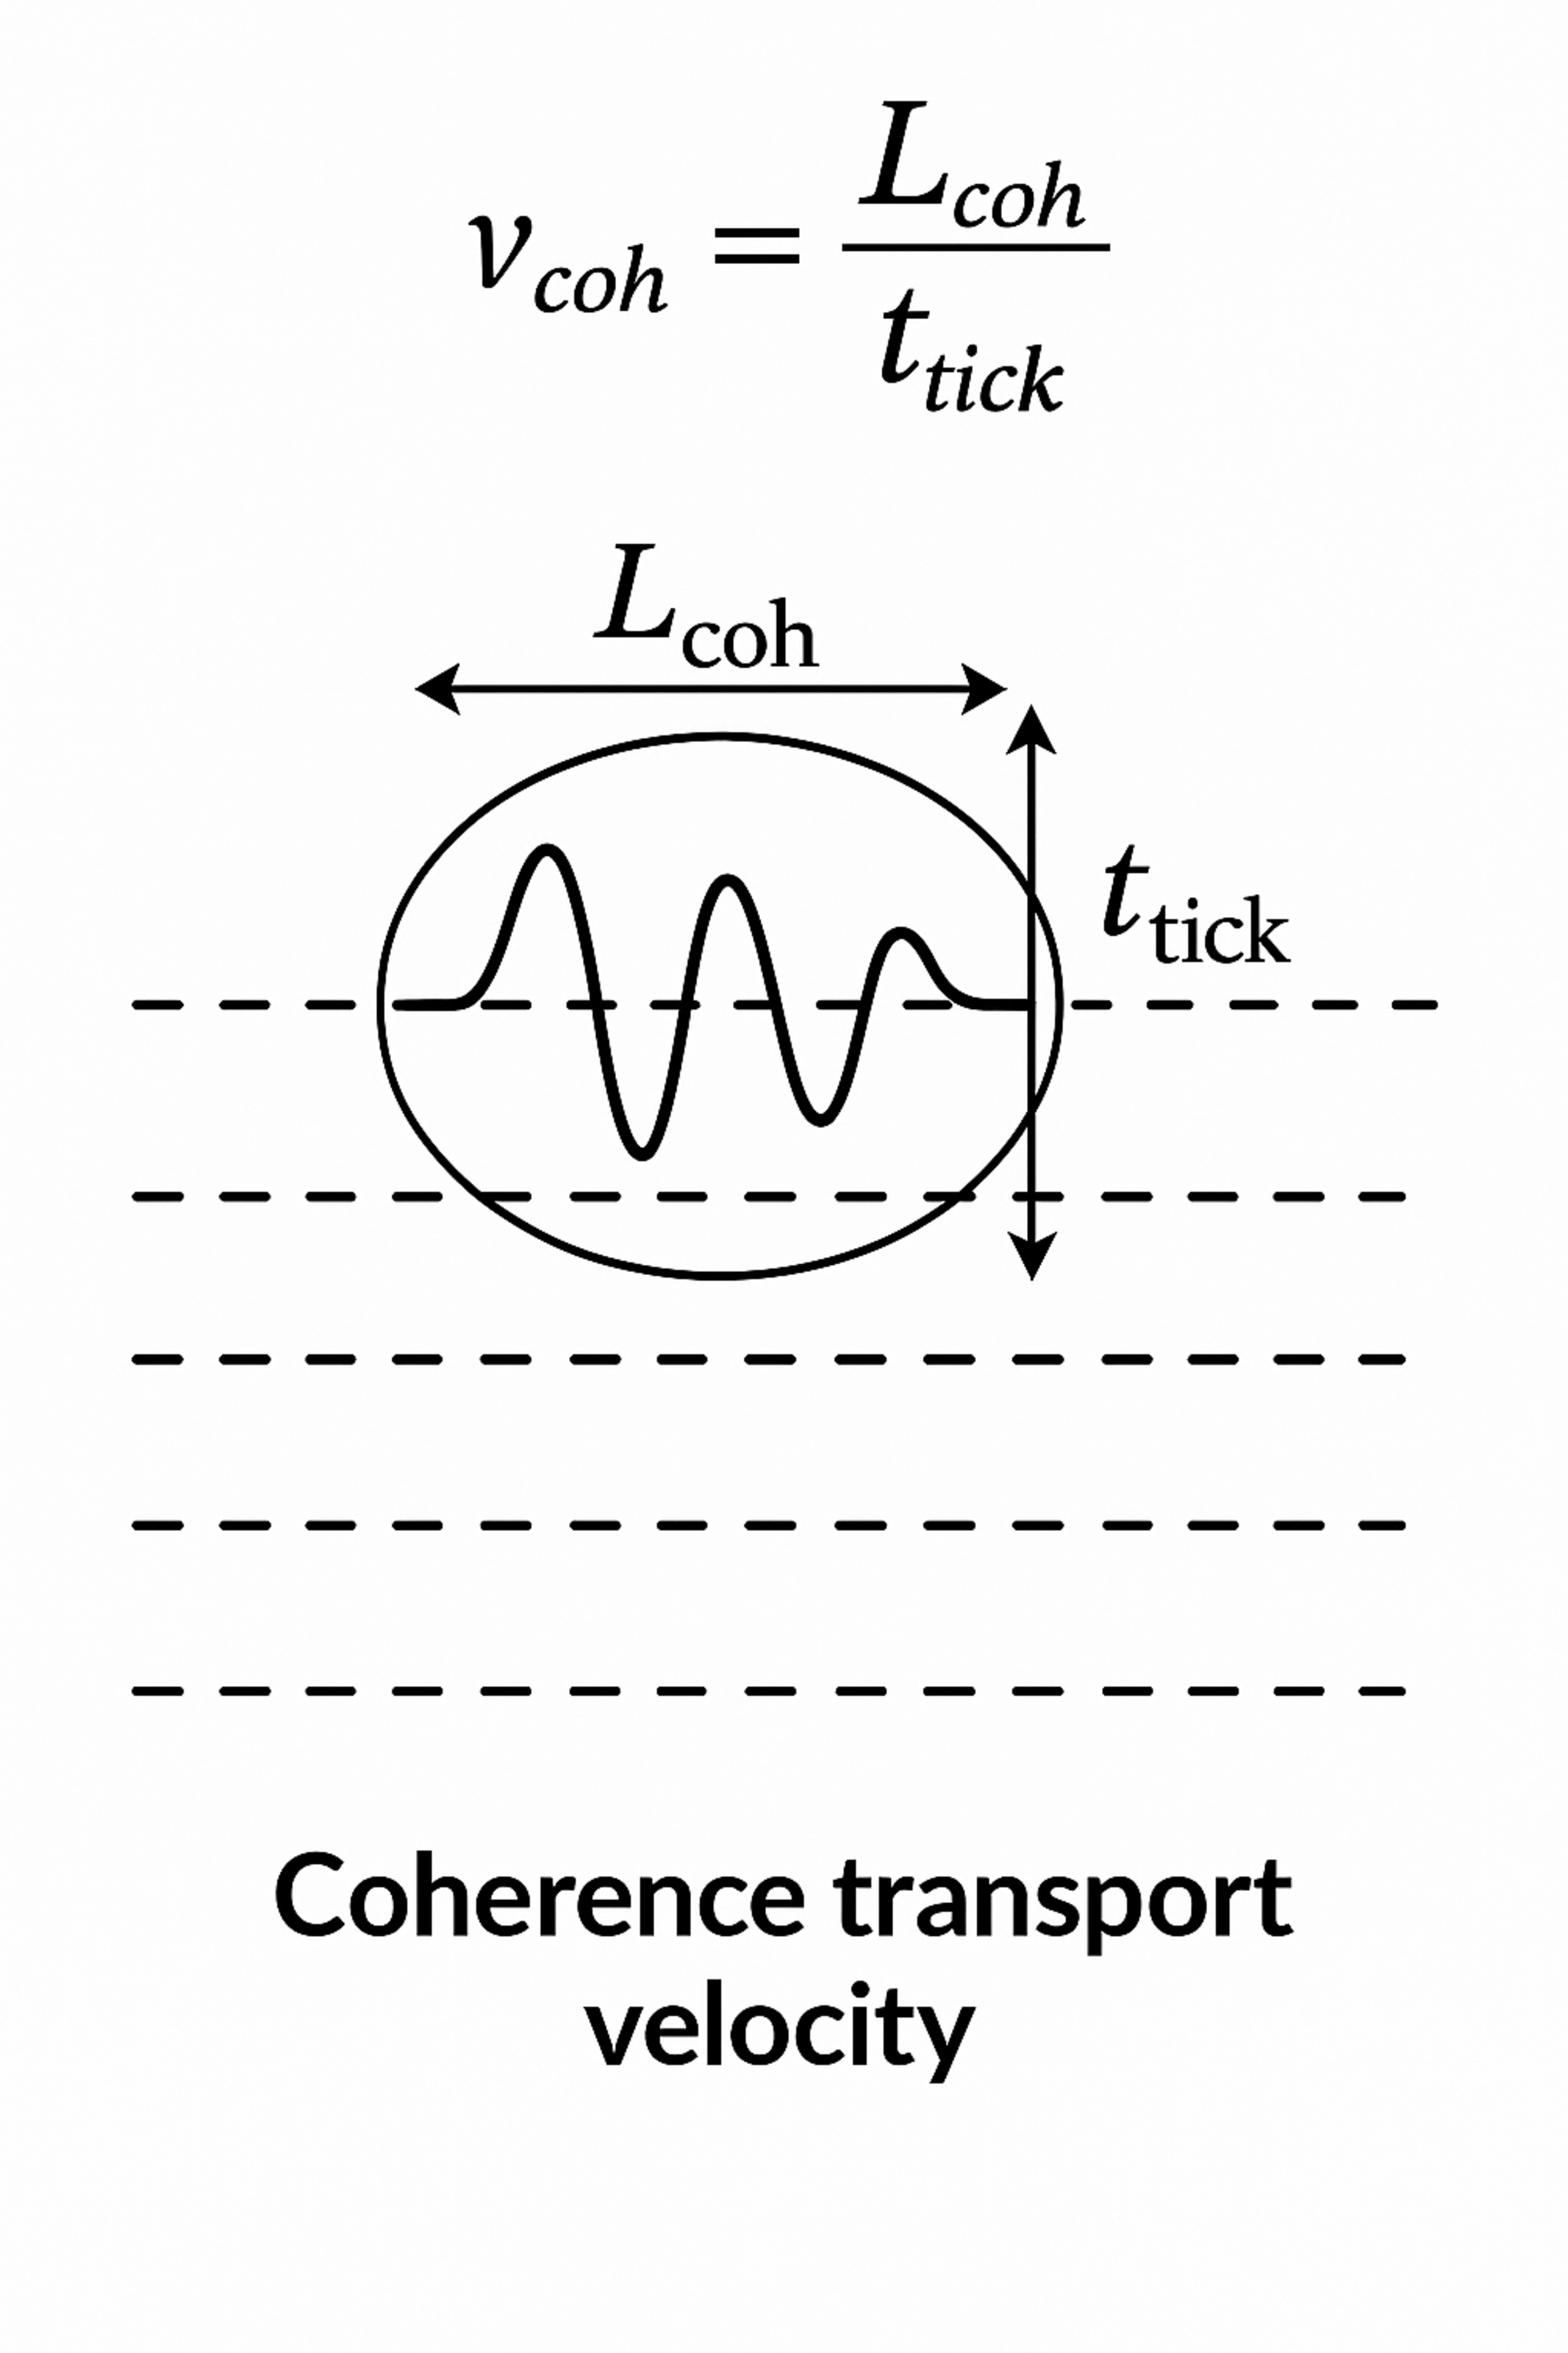
\includegraphics[width=0.6\textwidth]{figures/CTV.pdf}
    \caption{
    \textbf{Coherence Transport Velocity.} 
    In Quantum Substrate Dynamics (QSD), motion is governed not by geometric traversal, but by the scalar re-locking of coherence structures across the substrate. The coherence transport velocity is defined as \( v_{\text{coh}} = \frac{L_{\text{coh}}}{t_{\text{tick}}} \), where \( L_{\text{coh}} \) is the effective coherence envelope size and \( t_{\text{tick}} \) is the local scalar recovery interval. This expression sets the maximum apparent speed at which coherent structures can move through the substrate without violating causal re-locking constraints.
    }
    \label{fig:coherence-transport-velocity}
\end{figure}

This ontological shift allows for a more physically grounded understanding of what it means for an object to be in motion, to accelerate, or to remain still. Stillness and uniform motion are no longer opposites—they are structurally indistinguishable in the absence of a tension gradient. Motion only arises when the substrate is required to reconfigure a phase structure under scalar constraint, which is experienced macroscopically as acceleration, resistance, and energy cost.
%%%%%%%%%%%%%%%%%%%%%%%%%%%%%%%%%%%%%%%%%%%%%%%%%%%%%%%%
\subsection{Inertia as Coherence Reconfiguration Resistance}

In classical physics, inertia is treated as an intrinsic property of mass---a passive resistance to acceleration. However, within the Quantum Substrate Dynamics (QSD) framework, inertia emerges from the substrate’s active resistance to the reconfiguration of a coherence structure. It is not the mass that resists motion, but the substrate that resists rapid or misaligned phase re-locking.

A mass-phase structure is defined by a stable configuration of phase-locked scalar coherence within a conserved substrate region. When a force attempts to accelerate this structure, it imposes a directional demand on the boundary shell to re-lock into a new substrate region. This demand requires scalar reconfiguration across a gradient, which involves scalar recovery delay and energy expenditure. Inertia, then, is the measure of the substrate’s coherence drag---the energetic cost and time delay associated with displacing the structure’s boundary under phase continuity constraints.

Mathematically, the inertial response may be modeled as a rate-dependent resistance proportional to the local curvature and amplitude of the phase gradient at the mass boundary. Rather than viewing inertia as a fixed quantity tied to mass, QSD reframes it as a dynamic interaction between the structure and the substrate: the more complex the boundary, the greater the resistance to reconfiguration, and thus the greater the apparent inertia.

This interpretation naturally resolves the observed symmetry between acceleration and deceleration. In both cases, the substrate is being asked to reconfigure the coherence structure---the direction of motion change is irrelevant to the underlying mechanism. The inertial experience is the scalar response to imposed reconfiguration pressure, not a consequence of momentum being "lost" or "gained."

By treating inertia as a reconfiguration process, QSD eliminates the need for mass as a fundamental property. Instead, mass becomes a label for how difficult it is to re-lock a given phase structure under scalar constraint. This offers a substrate-level mechanism for understanding resistance to motion, while remaining compatible with classical measurements and relativistic consistency.

To formalize the substrate's resistance to coherence boundary reconfiguration, we propose a first-order inertial model:

\begin{equation}
    F_{\text{inertial}} \propto \kappa \cdot \frac{d}{dt} \nabla \theta(\vec{r}),
\end{equation}

where \( \nabla \theta(\vec{r}) \) is the local phase gradient at the coherence boundary, and \( \kappa \) is a substrate compliance constant that characterizes the drag imposed by scalar recovery delay. This expression captures the time-dependent structural response of the substrate to imposed acceleration.


%%%%%%%%%%%%%%%%%%%%%%%%%%%%%%%%%%%%%%%%%%
\subsection{Acceleration, Deceleration, and Momentum}

In the QSD framework, acceleration and deceleration are not fundamentally distinct phenomena. Both represent a deviation from uniform re-locking of a coherence structure and require scalar reconfiguration. From the substrate's perspective, changing motion in any direction imposes a demand on the local phase gradient, leading to a temporary deformation of the coherence shell. The direction of the change is irrelevant to the structural mechanism: what matters is that a re-lock event must occur at a different pace or into a new geometric alignment.

Momentum, in this view, is not a carried quantity but an expression of the substrate’s ongoing commitment to a reconfiguration path. It reflects the degree to which a coherence structure is already entangled with a directional scalar gradient. When a system is in motion, the substrate has already configured itself to support that coherence flow; interrupting or reversing it requires overcoming the stored phase alignment. This accounts for the persistence of motion and the energetic cost of stopping.

Mathematically, momentum can be reinterpreted as the integral of scalar re-locking activity over the coherence path:
\[
\vec{p}_{\text{QSD}} = \int_{\Omega} \rho(\vec{r}) \, \nabla \theta(\vec{r}) \, d^3r,
\]
where \( \rho(\vec{r}) \) is the coherence density, and \( \nabla \theta(\vec{r}) \) is the local phase gradient. This formulation captures both the directionality and the accumulated structural commitment of the mass-phase envelope as it moves through the substrate.

The energetic consequences of momentum are not stored in the mass, but in the substrate's geometric configuration. A sudden stop or impact leads to scalar rupture---the substrate can no longer maintain coherence continuity and must offload accumulated tension as heat, vibration, or deformation. This resolves the classical question of why collisions produce energy release even when no energy is “stored” in a moving object.

By reinterpreting acceleration, deceleration, and momentum as aspects of scalar reconfiguration within a conserved substrate, QSD provides a physically grounded mechanism for motion change. It preserves Newtonian outcomes in appropriate regimes, while replacing unexplained axioms with substrate-consistent structural dynamics.
%%%%%%%%%%%%%%%%%%%%%%%%%%%%%%%%%%%%%%%%%%
\subsection{Perceived Weight as Substrate Equilibrium Resistance}

In the classical view, weight is defined as the gravitational force acting on a mass: \( W = mg \), where \( g \) is the local gravitational field strength. This formulation describes what is measured, but does not explain what weight is in structural terms. Within the QSD framework, perceived weight arises from the substrate’s scalar tension gradient and the coherence structure’s resistance to being re-anchored into a lower-tension equilibrium.

Gravity in QSD is not a force field, but a coherence tension gradient within the substrate. Mass-phase structures immersed in such a gradient experience a directional preference for scalar re-locking toward regions of lower tension. Free-falling objects follow this gradient naturally, undergoing continuous re-locking without resistance; no internal deformation occurs, and thus no weight is perceived, see Figure \ref{fig:weight-denied-relock}.

\begin{figure}[H]
    \centering
    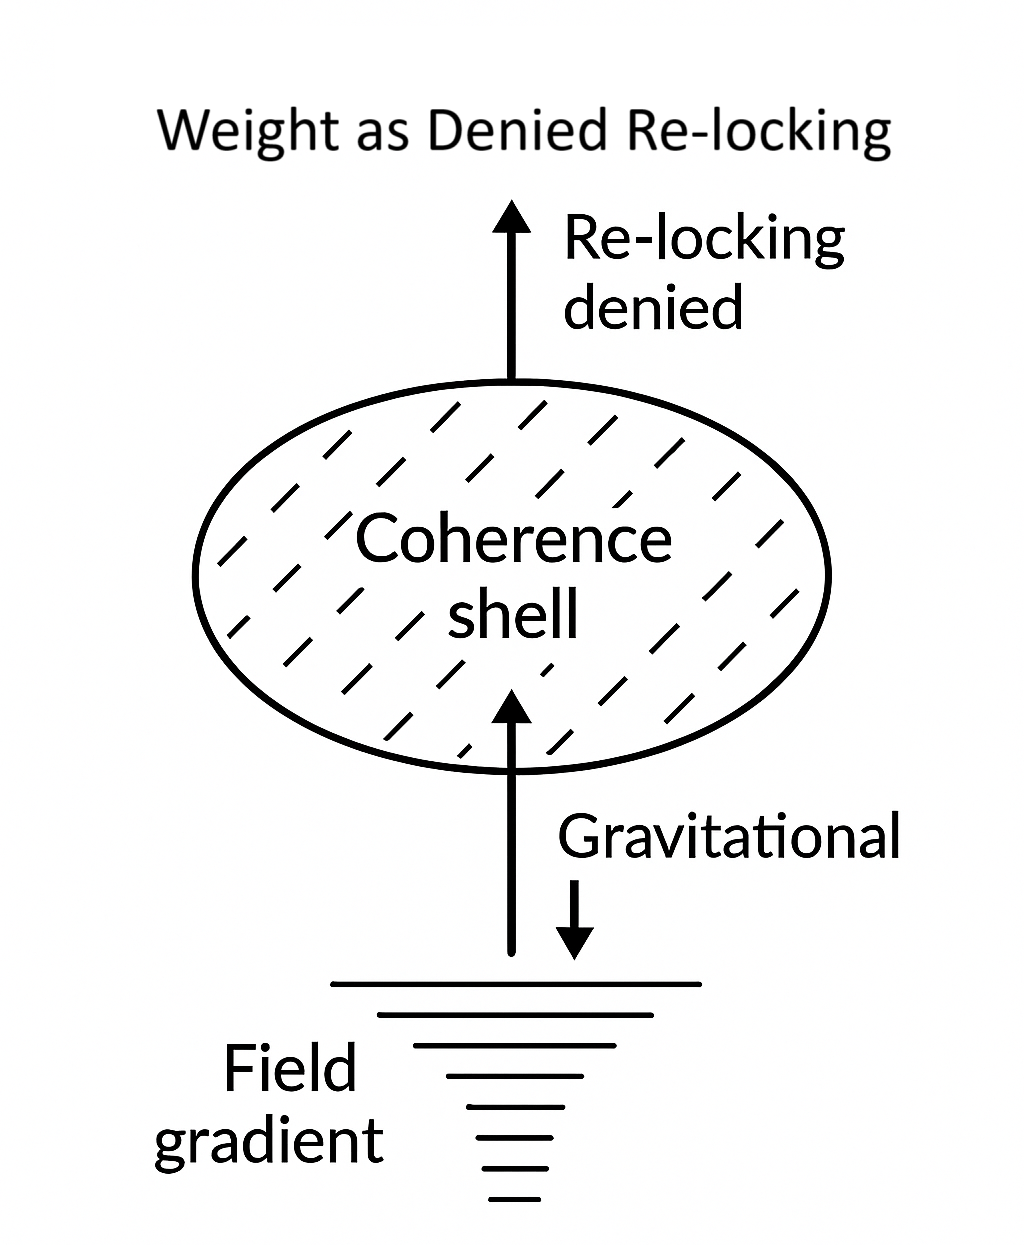
\includegraphics[width=0.5\textwidth]{figures/weight.png}
    \caption{
    \textbf{Weight as Denied Re-locking.}
    In the QSD framework, weight is not a force between masses but a structural phenomenon arising from coherence denial. A mass-phase coherence shell situated in a gravitational gradient attempts to re-lock into regions of lower scalar tension. When external constraints prevent this re-locking—such as contact with a surface—the substrate imposes a pushback against the denied direction. This denied reconfiguration manifests as weight: a scalar resistance to unfulfilled re-locking across a gradient. The gravitational vector reflects the substrate’s structural preference for re-lock alignment toward equilibrium.
    }
    \label{fig:weight-denied-relock}
\end{figure}


Weight only appears when a coherence structure is constrained against the gradient---such as when it is supported by a surface. In this case, the substrate continues to attempt re-locking the structure downward, but the coherence shell cannot resolve the tension gradient due to boundary opposition. This denial of equilibrium results in a continuous scalar pushback, experienced as weight. It is not a force transmitted through space, but the tension imposed by the substrate when a structure is held out of gradient-aligned motion.

This mechanism naturally explains why objects in free fall feel weightless: their scalar coherence is continuously re-locking in the gradient direction without interference. Likewise, it explains why astronauts in orbit experience microgravity despite remaining within Earth's gravitational field---their structures are in uninterrupted substrate alignment and do not resist equilibrium.

Weight, in QSD, is not an intrinsic interaction between two masses, but a local phenomenon resulting from the interruption of scalar gradient flow. It scales with the steepness of the coherence tension gradient and the coherence mass’s inability to reconfigure. This interpretation offers a structural origin for the sensation of weight, grounded entirely in substrate dynamics and conservation.

This scalar resistance also clarifies gravitational behavior without invoking attractive forces. In QSD, a mass-phase structure deforms the substrate by introducing a coherence tension gradient. This gradient represents an elevated strain energy profile that the substrate seeks to resolve. When a second coherence structure enters this gradient, it experiences a re-locking tendency toward regions of lower substrate tension—not because it is pulled, but because the substrate permits structural change in the direction of minimal deformation cost. In this view, motion in a gravitational field arises from the substrate’s preference for coherence resolution, not external force, preserving both conservation and causal continuity.

To express weight as a consequence of substrate tension gradient resistance, we define the scalar push back integral:

\begin{equation}
    W = \int_{\Omega} \rho(\vec{r}) \cdot \nabla \Phi_{\text{coh}}(\vec{r}) \, d^3r,
\end{equation}

where \( \rho(\vec{r}) \) is the local coherence density and \( \Phi_{\text{coh}}(\vec{r}) \) is the scalar coherence potential describing tension alignment within the substrate. This expression captures the substrate’s attempt to resolve mass-phase structures into equilibrium and formalizes weight as the reaction to denied scalar re-locking in a downward gradient.

In the Quantum Substrate Dynamics (QSD) framework, Newton’s second law is not discarded, but reinterpreted as a large-scale approximation of substrate resistance to coherence reconfiguration. The classical formulation \( F = ma \) becomes a surface-level expression of the structural tension that arises when a mass-phase coherence structure is denied alignment with a scalar tension gradient. Acceleration does not result from force acting on mass, but from a directional increase in scalar re-locking demand. When this reconfiguration is obstructed—such as when a mass is supported against a gravitational gradient—the substrate imposes a pushback proportional to both the steepness of the scalar potential (\( \nabla \Phi_{\text{coh}} \)) and the structure’s resistance to re-locking. In this view, what we interpret as "force" is actually substrate tension attempting to complete a denied scalar reconfiguration, and "mass" is the scalar reconfiguration difficulty associated with a coherence envelope. Newton’s law is thus reframed not as a fundamental equation of motion, but as an emergent descriptor of a deeper substrate effort to resolve phase misalignment under tension.



%%%%%%%%%%%%%%%%%%%%%%%%%%%%%%%%%%%%%%%%%%
\subsection{Rotation and Angular Momentum}

Within classical mechanics, angular momentum is treated as a conserved quantity: the product of a body’s moment of inertia and its angular velocity. This approach successfully predicts macroscopic rotational behavior, but offers no structural account of what angular momentum is or why rotating systems resist directional change. In Quantum Substrate Dynamics (QSD), angular momentum arises from the substrate’s conservation of curved phase flow. A rotating mass-phase structure induces persistent coherence deformation, and angular momentum is the measure of the substrate’s ongoing commitment to maintain this curved re-locking path.

Rotation differs fundamentally from linear motion. In uniform linear motion, scalar re-locking can occur without tension imbalance if the substrate gradient is flat. In contrast, rotation imposes continuous curvature on the coherence shell, requiring re-locking into geometrically misaligned adjacent zones. This re-locking under curvature creates structural strain in the substrate, which resists rapid change and demands scalar recovery to maintain.

The substrate stores this deformation as a standing torsional pattern---a curved memory---and any attempt to alter the rotation axis results in additional reconfiguration demand. This explains gyroscopic resistance: the substrate is actively conserving the angular phase geometry, and directional change requires it to restructure the coherence loop, which is energetically expensive.

Angular momentum in QSD is not a vector carried by the object, but a structural flow of phase within the substrate:
\[
\vec{L}_{\text{QSD}} = \int_{\Omega} \rho(\vec{r}) \left( \vec{r} \times \nabla \theta(\vec{r}) \right) d^3r,
\]
where \( \rho(\vec{r}) \) is the coherence density and \( \nabla \theta(\vec{r}) \) is the local phase gradient tangent to the curved motion path. This integral reflects the stored angular deformation, not just a kinematic property of mass.

Rotational motion also introduces persistent scalar recovery lag. The substrate cannot instantly recover from curved re-locking cycles, and this results in energy offload over time. Even uniform rotation leads to measurable thermal loss due to scalar rupture and jitter at the coherence boundary. Rapid directional changes, such as tilting a spinning gyroscope, accelerate this offload process, causing faster spin-down and increased heating—effects not explained by classical friction models.

The scalar recovery lag resulting from persistent curved motion can be modeled as an offload power function:

\begin{equation}
    P_{\text{offload}}(t) = \gamma \cdot \frac{\Delta E_{\text{torsion}}}{\tau},
\end{equation}

where \( \Delta E_{\text{torsion}} \) is the accumulated torsional strain energy stored in the coherence structure, \( \tau \) is the scalar recovery timescale, and \( \gamma \) is a coupling factor relating tension offload to measurable thermal output. This relationship provides a falsifiable prediction: that post-rotation heating scales with coherence strain and scalar pacing lag, even in isolated systems.


In QSD, angular momentum is structurally conserved but energetically costly. The longer or faster a body spins, the more curvature memory is invested in the substrate, and the more difficult it becomes to alter or interrupt that motion. This reframe explains gyroscopic stability, spin decay, and inertial resistance from first principles, without invoking mass as a primitive or abstract conservation rules, see Figure \ref{fig:inertial-resistance}.

\begin{figure}[H]
    \centering
    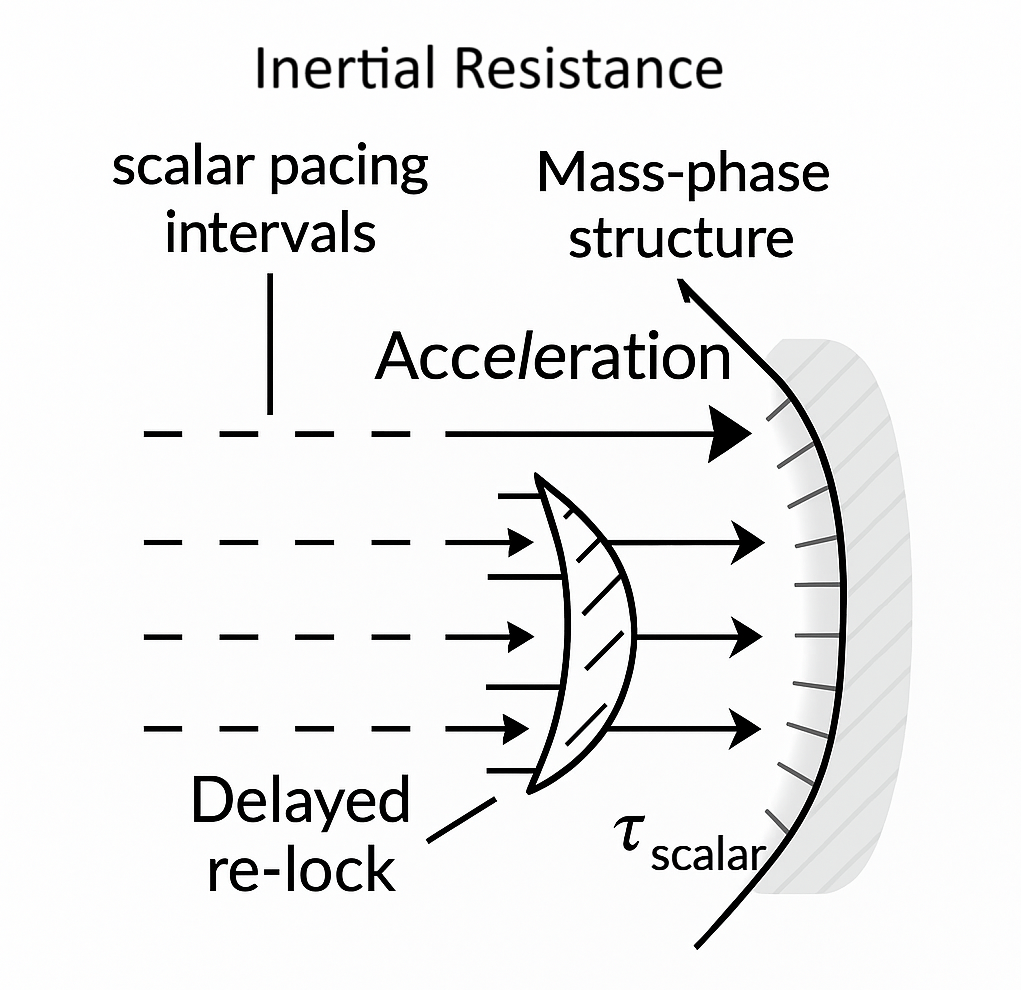
\includegraphics[width=0.6\textwidth]{figures/inertia.png}
    \caption{
    \textbf{Inertial Resistance and Scalar Pacing.}
    In Quantum Substrate Dynamics (QSD), inertial resistance arises from the delay between scalar pacing intervals and the structural reconfiguration of a mass-phase boundary. As a coherence structure accelerates, its re-locking into the substrate becomes desynchronized, resulting in a temporary lag or deformation. This delay, represented by the scalar recovery time \( \tau_{\text{scalar}} \), defines the pacing-limited resistance experienced as inertia. The substrate cannot re-lock the boundary faster than its causal capacity permits, making inertia a time-constrained response rather than an intrinsic mass property.
    }
    \label{fig:inertial-resistance}
\end{figure}

%%%%%%%%%%%%%%%%%%%%%%%%%%%%%%%%%%%%%%%%%%
\subsection{Energy and Motion}

In classical physics, energy is treated as a transferable and often conserved quantity that can be stored in objects as kinetic or potential forms. Within the QSD framework, energy is reinterpreted not as a stored substance or scalar value, but as the act of reconfiguring phase-coherent structures in the substrate. All energy is procedural---it arises when coherence structures are deformed, displaced, or re-locked under substrate tension constraints.

Motion does not inherently carry energy. A coherence structure in uniform motion, aligned with a tension-neutral scalar gradient, induces no offload or substrate deformation, and therefore has no energetic expression. Energy expenditure only arises when motion changes: during acceleration, deceleration, rotation, or any event requiring reconfiguration of the boundary shell. In these cases, scalar re-locking fails to occur seamlessly, and the substrate must expend structural effort to maintain continuity or repair phase misalignment.

Kinetic energy, in this context, is not something “possessed” by a moving object. It is a measure of the amount of structural deformation the substrate is sustaining to preserve the coherence of a motion path under scalar timing constraints. Similarly, potential energy is not stored in position, but reflects the substrate's readiness to resolve a phase structure into a lower-tension configuration---as in the case of a mass held above a coherence gradient.

Thermal energy arises when the substrate fails to re-lock cleanly, resulting in scalar offload events. These events dissipate tension in the form of low-scale coherence jitter, which appears macroscopically as heat. This explains why mechanical systems warm during repeated deformation, even in the absence of friction: the scalar memory becomes saturated and releases energy as incoherent boundary vibration.

Energy conservation in QSD is preserved structurally. What is traditionally considered "conserved energy" is instead the continuous redistribution of phase tension and scalar recovery effort. When a mass-phase structure comes to rest, its energy is not stored in the object, but has been offloaded into the substrate through structural reconfiguration and recovery delay. This offers a physical explanation for energy transformation and loss, without invoking abstract potentials or hidden reservoirs.

Thus, QSD reframes energy as an emergent behavior of substrate tension dynamics. Motion is energetically neutral unless it requires change; acceleration, deformation, or constrained re-locking generate scalar tension, which the substrate must resolve. Energy is not stored in moving things---it is the substrate’s cost of keeping coherence intact when structural continuity is disrupted.

%%%%%%%%%%%%%%%%%%%%%%%%%%%%%%%%%%%%%%%%%%
\subsection{Compatibility with Classical Physics}

The Quantum Substrate Dynamics (QSD) framework reinterprets motion, inertia, and energy as structural outcomes of scalar coherence dynamics, rather than as primitive concepts. Despite this shift in ontology, QSD remains fully compatible with classical physics in its predictive domain. The classical equations of motion, Newtonian mechanics, and relativistic kinematics all emerge as effective descriptions of substrate behavior in the appropriate limits.

QSD preserves conservation of energy, momentum, and angular momentum, but reframes these as expressions of coherence preservation and substrate symmetry. Inertial reference frame equivalence, as formulated by Einstein, is naturally explained by the substrate’s scalar neutrality in tension-balanced regions. Lorentz invariance is upheld through the scalar recovery constraint, which enforces causal propagation and ensures that no coherence structure can exceed the substrate’s re-locking rate.

Apparent paradoxes in classical motion---such as the equivalence of rest and uniform velocity, the energetic consequences of impact, and the source of inertial resistance---are resolved structurally in QSD without altering observed behavior. Newton’s laws are recovered as large-scale summaries of substrate response: force emerges as imposed curvature, acceleration as coherence reconfiguration, and mass as phase resistance geometry.

General relativity’s treatment of gravity as spacetime curvature finds a coherent analog in QSD: gravitational effects are modeled as scalar tension gradients within a conserved coherence field. This results in equivalent predictions for orbital motion, free fall, and gravitational time dilation, while offering a mechanism rooted in phase continuity rather than geometric postulation.

Importantly, QSD does not negate quantum or classical frameworks, but provides a deeper substrate from which their behavior can be derived. It respects the successes of legacy physics while offering a structural explanation for quantities that were previously defined only mathematically. In this way, QSD supports continuity with established theory while extending its conceptual foundation to include causally coherent, falsifiable mechanisms.
%%%%%%%%%%%%%%%%%%%%%%%%%%%%%%%%%%%%%%%%%%
\subsection{Reframing Motion Through Structure}

The results presented in this paper invite a fundamental shift in how motion, inertia, and momentum are understood—not as axiomatic quantities, but as emergent behaviors arising from phase-coherent structures embedded in a conserved substrate. The QSD framework provides a physically grounded mechanism for phenomena that classical and relativistic models treat as primitive: inertia becomes coherence drag, motion becomes scalar re-locking, and momentum becomes the substrate’s directional commitment to ongoing structural flow.

This reframing does not reject existing physics but reveals the continuity beneath it. Classical laws remain valid as high-level summaries, and relativistic constraints are naturally preserved through the scalar propagation limits imposed by the substrate. The advantage of the QSD approach lies in its ability to assign physical meaning to otherwise unexplained postulates, offering a structural cause for inertial resistance, the indistinguishability of rest and uniform motion, and the observable symmetry between acceleration and deceleration.

The framework also provides new interpretations for thermal effects and apparent energy loss in rotating systems. Scalar offload during coherence reconfiguration leads to heating, even in idealized vacuum conditions—an effect long observed but only loosely attributed to internal friction or mechanical damping. QSD shows that this heat arises from incomplete scalar recovery during persistent curvature, offering a testable prediction that rotational systems will exhibit asymmetric post-stop thermal output proportional to angular strain and tilt frequency.

Moreover, by placing coherence structure at the foundation of all motion, QSD suggests that even fundamental quantities like mass and energy are not intrinsic but procedural—dependent on how the substrate stores and resolves phase tension. This has implications not only for classical mechanics, but for how quantum systems, fields, and spacetime geometry are modeled at their most fundamental level.

This work represents a step toward a more physically honest formulation of motion, one rooted in substrate logic rather than abstracted forces. It opens the door to new experimental investigations, including scalar-based inertial detection, post-rotation thermal imaging, and substrate-driven transport mechanisms—all grounded in coherence conservation. The aim is not to replace the successful tools of physics, but to give them a deeper foundation: one in which motion, inertia, and structure are inseparable aspects of the same underlying reality.

%%%%%%%%%%%%%%%%%%%%%%%%%%%%%%%%%%%%%%%%%%
\section{Conclusion}
%%%%%%%%%%%%%%%%%%%%%%%%%%%%%%%%%%%%%%%%%%
This work has presented a structural reinterpretation of motion, inertia, and momentum within the framework of Quantum Substrate Dynamics (QSD). By modeling mass-phase structures as coherence knots embedded in a conserved substrate, we have shown that motion is not traversal through space, but the scalar re-locking of phase across a coherence-supporting medium. Inertia emerges not from intrinsic mass, but from the energetic cost of reconfiguring a stable boundary under scalar constraint. Momentum is redefined as the directional commitment of the substrate to maintain a coherence path, and weight arises from the tension experienced when re-locking is denied in the presence of a gravitational gradient.

Rotational motion was shown to impose persistent substrate deformation, leading to irreversible scalar strain and measurable thermal effects—even in the absence of classical friction. Angular momentum is recast as a conserved curvature memory, and the structural basis of gyroscopic resistance is derived from the substrate's commitment to maintain curved phase geometry. These interpretations provide physically intuitive, testable explanations for long-standing classical assumptions, while remaining fully consistent with conservation laws and Lorentz invariance.

Throughout, no classical principle was violated; instead, each was reframed as a projection of deeper coherence structure. What began as a reexamination of motion resulted in a comprehensive structural ontology for mass, acceleration, resistance, and energy transfer. The QSD framework transforms motion from a kinematic description into a process of scalar continuity and phase preservation, offering a more causally transparent and physically grounded alternative to traditional mechanics.

This reinterpretation opens new possibilities for modeling mechanical systems, inertial effects, and thermal dynamics from first principles. It also lays the foundation for future investigations into coherence-bound transport, rotational entropy, and the role of scalar recovery in quantum and macroscopic systems. By grounding motion in structure rather than assumption, QSD reclaims inertia and momentum as the conserved consequences of an active, coherent substrate.



%%%%%%%%%%%%%%%%%%%%%%%%%%%%%%%%%%%%%%%%%%
\vspace{6pt} 

%%%%%%%%%%%%%%%%%%%%%%%%%%%%%%%%%%%%%%%%%%
%% optional
%\supplementary{The following supporting information can be downloaded at:  \linksupplementary{s1}, Figure S1: title; Table S1: title; Video S1: title.}

% Only for journal Methods and Protocols:
% If you wish to submit a video article, please do so with any other supplementary material.
% \supplementary{The following supporting information can be downloaded at: \linksupplementary{s1}, Figure S1: title; Table S1: title; Video S1: title. A supporting video article is available at doi: link.}

% Only used for preprtints:
% \supplementary{The following supporting information can be downloaded at the website of this paper posted on \href{https://www.preprints.org/}{Preprints.org}.}

% Only for journal Hardware:
% If you wish to submit a video article, please do so with any other supplementary material.
% \supplementary{The following supporting information can be downloaded at: \linksupplementary{s1}, Figure S1: title; Table S1: title; Video S1: title.\vspace{6pt}\\
%\begin{tabularx}{\textwidth}{lll}
%\toprule
%\textbf{Name} & \textbf{Type} & \textbf{Description} \\
%\midrule
%S1 & Python script (.py) & Script of python source code used in XX \\
%S2 & Text (.txt) & Script of modelling code used to make Figure X \\
%S3 & Text (.txt) & Raw data from experiment X \\
%S4 & Video (.mp4) & Video demonstrating the hardware in use \\
%... & ... & ... \\
%\bottomrule
%\end{tabularx}
%}

\section*{Statements and Declarations}
\subsection*{Funding}  
The author received no financial support for the research, authorship, or publication of this article.
The author has no relevant financial or non-financial interests to disclose.

\subsection*{Competing Interests}  
The author declares no competing interests.

\subsection*{Author Contributions}  
The author solely conceived, developed, and wrote the manuscript, including all theoretical content, references, and formatting.

\subsection*{Data Availability}  
No datasets were generated or analyzed during the current study. All references are publicly available.

\subsection*{Ethical Approval}  
Not applicable.


%%%%%%%%%%%%%%%%%%%%%%%%%%%%%%%%%%%%%%%%%%
%% Optional

%% Only for journal Encyclopedia
%\entrylink{The Link to this entry published on the encyclopedia platform.}

\abbreviations{Abbreviations}{
The following abbreviations are used in this manuscript:
\\

\noindent
\begin{tabular}{@{}ll}
QSD   & Quantum Substrate Dynamics \\
\( c_s \) & Scalar coherence recovery speed (temporal mode) \\
\( c_t \) & Transverse coherence propagation speed (spatial mode) \\
\( L_0 \) & Baseline coherence length at rest \\
\( L_{\text{coh}}(r) \) & Curvature-stretched coherence support length \\
\( v \) & Apparent velocity relative to substrate \\
\( v_{\text{coh}} \) & Coherence transport velocity \( = \frac{L_{\text{coh}}}{t_{\text{tick}}} \) \\
\( t_{\text{tick}} \) & Local scalar recovery interval (effective time tick) \\
\( t_0 \) & Tick duration at rest (baseline tick) \\
\( \kappa \) & Substrate compliance constant (resistance to boundary deformation) \\
\( \theta(\vec{r}) \) & Local coherence phase at position \( \vec{r} \) \\
\( \rho(\vec{r}) \) & Coherence density distribution \\
\( F_{\text{inertial}} \) & Inertial response force under reconfiguration stress \\
\( P_{\text{offload}}(t) \) & Scalar thermal offload power over time \\
\( \Delta E_{\text{torsion}} \) & Accumulated torsional energy due to rotational strain \\
\( \tau \) & Scalar recovery lag timescale \\
\( \gamma \) & Lorentz factor (compatible structural form) \\
GPS  & Global Positioning System \\
SR   & Special Relativity \\
GR   & General Relativity \\
\end{tabular}

}



%%%%%%%%%%%%%%%%%%%%%%%%%%%%%%%%%%%%%%%%%%
%% Optional
\appendixtitles{no} % Leave argument "no" if all appendix headings stay EMPTY (then no dot is printed after "Appendix A"). If the appendix sections contain a heading then change the argument to "yes".
\appendixstart
\appendix
%%%%%%%%%%%%%%%%%%%%%%%%%%%%%%%%%%%%%%%%%%%%%%%
\section[\appendixname~\thesection]{}
\subsection[\appendixname~\thesubsection]{Canonical QSD Motion Equations}
%%%%%%%%%%%%%%%%%%%%%%%%%%%%%%%%%%%%%%%%%%%%%%

The following expressions summarize the core structural relationships introduced in this paper. Each equation reflects a specific substrate-level mechanism related to motion, inertia, momentum, energy dissipation, or gravitational resistance, reformulated within the Quantum Substrate Dynamics (QSD) framework.

\subsubsection{Inertial Resistance}
Inertia arises from resistance to reconfiguring the coherence boundary under phase-gradient deformation:
\begin{equation}
    F_{\text{inertial}} \propto \kappa \cdot \frac{d}{dt} \nabla \theta(\vec{r}),
\end{equation}
where \( \kappa \) is the substrate compliance constant and \( \nabla \theta(\vec{r}) \) is the local phase gradient.

\subsubsection{Momentum as Coherence Path Commitment}
Momentum is defined not as mass times velocity, but as integrated structural commitment to directional scalar flow:
\begin{equation}
    \vec{p}_{\text{QSD}} = \int_{\Omega} \rho(\vec{r}) \, \nabla \theta(\vec{r}) \, d^3r,
\end{equation}
where \( \rho(\vec{r}) \) is the coherence density and \( \nabla \theta(\vec{r}) \) is the local phase gradient.

\subsubsection{Rotational Offload Power}
Rotational motion induces coherence strain, which offloads thermally as scalar recovery fails:
\begin{equation}
    P_{\text{offload}}(t) = \gamma \cdot \frac{\Delta E_{\text{torsion}}}{\tau},
\end{equation}
where \( \Delta E_{\text{torsion}} \) is accumulated torsional energy, \( \tau \) is the scalar recovery timescale, and \( \gamma \) is an offload coupling factor.

\subsubsection{Weight from Gradient Tension}
Weight emerges from scalar pushback when re-locking is denied in a downward tension gradient:
\begin{equation}
    W = \int_{\Omega} \rho(\vec{r}) \cdot \nabla \Phi_{\text{coh}}(\vec{r}) \, d^3r,
\end{equation}
where \( \Phi_{\text{coh}}(\vec{r}) \) is the coherence tension potential.

\subsubsection{Coherence Transport Velocity}
Motion is constrained not by geometric traversal, but by the rate of allowable re-locking across scalar intervals:
\begin{equation}
    v_{\text{coh}} = \frac{L_{\text{coh}}}{t_{\text{tick}}},
\end{equation}
where \( L_{\text{coh}} \) is the coherence envelope size and \( t_{\text{tick}} \) is the scalar recovery interval.

\vspace{1em}

These equations serve as the foundational structural mechanics for QSD-based motion modeling and are intended to replace kinematic postulates with physically grounded substrate behavior.

%%%%%%%%%%%%%%%%%%%%%%%%%%%%%%%%%%%%%%%%%%%%%%

%%%%%%%%%%%%%%%%%%%%%%%%%%%%%%%%%%%%%%
%\subsubsection{SUB A}
%%%%%%%%%%%%%%%%%%%%%%%%%%%%%%%%%%%%%%

%%%%%%%%%%%%%%%%%%%%%%%%%%%%%%%%%%%%%%%%%%%%%%%
%\section[\appendixname~\thesection]{}
%\subsection[\appendixname~\thesubsection]{APP B}
%%%%%%%%%%%%%%%%%%%%%%%%%%%%%%%%%%%%%%%%%%%%%%%

%\subsubsection{SUB B}

%%%%%%%%%%%%%%%%%%%%%%%%%%%%%%%%%%%%%%%%%%
%\isPreprints{} % If the paper is ``preprints'', please uncomment this parenthesis.
%\printendnotes[custom] % Un-comment to print a list of endnotes

\reftitle{References}

% Please provide either the correct journal abbreviation (e.g. according to the “List of Title Word Abbreviations” http://www.issn.org/services/online-services/access-to-the-ltwa/) or the full name of the journal.
% Citations and References in Supplementary files are permitted provided that they also appear in the reference list here. 

%=====================================
% References, variant A: external bibliography
%=====================================
% \bibliography{your_external_BibTeX_file}

%=====================================
% References, variant B: internal bibliography
%=====================================

% ACS format
\isAPAandChicago{}{%
\begin{thebibliography}{999}
% Reference 
\bibitem{bush2025}
\textbf{Preprint.} Bush, M. (2025). Quantum Substrate Dynamics (QSD): A Relativistic Field Model of Emergent Mass, Inertia and Gravity. \textit{Preprints}, 2025060988. \url{https://doi.org/10.20944/preprints202506.0988.v1}
% reference
\bibitem{bush-planck-2025}
\textbf{Preprint.} Bush, M. (2025). Planck’s Constant Physically Derived Through Quantum Substrate Dynamics: A Mode-Ratio and Offload-Based Origin for Quantization and Temporal Structure. \textit{Preprints}, 2024010211. \url{https://doi.org/10.20944/preprints202401.0211.v1}
% Reference 
\bibitem{bush-coherence}
Bush, M. The Coherence Envelope: Defining the Minimum Structural Unit of Action in Quantum Substrate Dynamics. {\em Preprints} {\bf 2025}, \url{https://doi.org/10.20944/preprints202506.2353.v1}.
% Reference 
\bibitem{bush-planck-ep}
Bush, M. Planck Energy as Collapse Limit: A Structural Interpretation of $E_P$ in Quantum Substrate Dynamics. {\em Preprints} {\bf 2025}, \url{https://doi.org/10.20944/preprints202507.0080.v1}.
% Reference 
\bibitem{planck1901}
\textbf{Journal article.} Planck, M. (1901). On the Law of Distribution of Energy in the Normal Spectrum. \textit{Annalen der Physik}, 4(553–563). \url{https://doi.org/10.1002/andp.19053221004}
% Reference 
\bibitem{einstein1905} 
\textbf{Journal article.} Einstein, A. (1905). On the electrodynamics of moving bodies. \textit{Annalen der Physik}, 322(10), 891–921. \url{https://doi.org/10.1002/andp.19053221004}
% Reference 
\bibitem{einstein1915} 
\textbf{Journal article.} Einstein, A. (1915). The field equations of gravitation. \textit{Sitzungsberichte der Preussischen Akademie der Wissenschaften}.
% Reference 
\bibitem[Ashby(2003)]{ashby-gps}
Ashby, N. Relativity in the Global Positioning System. {\em Living Rev. Relativ.} {\bf 2003}, {\em 6}, 1--50. \url{https://doi.org/10.12942/lrr-2003-1}.
% Reference
\bibitem[Bailey et al.(1977)]{bailey-muon}
Bailey, J.; Borer, K.; Combley, F.; Drumm, H.; Krienen, F.; Picasso, E.; von Ruden, W.; Farley, F.J.M.; Field, J.H. Measurements of relativistic time dilatation for positive and negative muons in a circular orbit. {\em Nature} {\bf 1977}, {\em 268}, 301--305. \url{https://doi.org/10.1038/268301a0}.
% reference
\bibitem[Everitt et al.(2011)]{gp-b}
Everitt, C.W.F.; et al. Gravity Probe B: Final Results of a Space Experiment to Test General Relativity. {\em Phys. Rev. Lett.} {\bf 2011}, {\em 106}, 221101. \url{https://doi.org/10.1103/PhysRevLett.106.221101}.

\bibitem[Chua et al.(2018)]{rotational-heating}
Chua, S.K.; et al. Thermal Noise in Precision Rotational Measurements. {\em Rev. Sci. Instrum.} {\bf 2018}, {\em 89}, 104501. \url{https://doi.org/10.1063/1.5042276}.


\end{thebibliography}
}

% Chicago format (Used for journal: arts, genealogy, histories, humanities, jintelligence, laws, literature, religions, risks, socsci)
\isChicagoStyle{%
\begin{thebibliography}{999}
% Reference 1
%\bibitem[Aranceta-Bartrina(1999a)]{ref-journal}
%Aranceta-Bartrina, Javier. 1999a. Title of the cited article. \textit{Journal Title} %6: 100--10.
% Reference 2

\end{thebibliography}
}{}

% APA format (Used for journal: admsci, behavsci, businesses, econometrics, economies, education, ejihpe, games, humans, ijfs, journalmedia, jrfm, languages, psycholint, publications, tourismhosp, youth)
\isAPAStyle{%
\begin{thebibliography}{999}
% Reference 1
%\bibitem[\protect\citeauthoryear{Azikiwe \BBA\ Bello}{{2020a}}]{ref-journal}
%Azikiwe, H., \& Bello, A. (2020a). Title of the cited article. \textit{Journal Title}, \textit{Volume}(Issue), 
%Firstpage--Lastpage/Article Number.

\end{thebibliography}
}{}

% If authors have biography, please use the format below
%\section*{Short Biography of Authors}
%\bio
%{\raisebox{-0.35cm}{\includegraphics[width=3.5cm,height=5.3cm,clip,keepaspectratio]{Definitions/author1.pdf}}}
%{\textbf{Firstname Lastname} Biography of first author}
%
%\bio
%{\raisebox{-0.35cm}{\includegraphics[width=3.5cm,height=5.3cm,clip,keepaspectratio]{Definitions/author2.jpg}}}
%{\textbf{Firstname Lastname} Biography of second author}

% For the MDPI journals use author-date citation, please follow the formatting guidelines on http://www.mdpi.com/authors/references
% To cite two works by the same author: \citeauthor{ref-journal-1a} (\citeyear{ref-journal-1a}, \citeyear{ref-journal-1b}). This produces: Whittaker (1967, 1975)
% To cite two works by the same author with specific pages: \citeauthor{ref-journal-3a} (\citeyear{ref-journal-3a}, p. 328; \citeyear{ref-journal-3b}, p.475). This produces: Wong (1999, p. 328; 2000, p. 475)

%%%%%%%%%%%%%%%%%%%%%%%%%%%%%%%%%%%%%%%%%%
%% for journal Sci
%\reviewreports{\\
%Reviewer 1 comments and authors’ response\\
%Reviewer 2 comments and authors’ response\\
%Reviewer 3 comments and authors’ response
%}
%%%%%%%%%%%%%%%%%%%%%%%%%%%%%%%%%%%%%%%%%%
\PublishersNote{}
%\isPreprints{} % If the paper is ``preprints'', please uncomment this parenthesis.
\end{document}

